%!TEX root=document.tex

\section{Introduction}
\label{sec:introduction}


Data visualization is one of the most common techniques for identifying 
trends and finding anomalies in data.
However, with high-dimensional datasets, identifying visualizations that 
effectively present interesting variations or patterns in the data is a non-trivial task:  a
user may have to plot thousands of pairs of attributes against each other 
before arriving at one that shows something valuable, optimizing for a range of visualization 
types, aesthetic features, and more.

%The hope is that these recommendations, combined with the current interactivity and ease of use of visualization 
%software, can help analysts quickly glean insights form the data.

In this paper, we tackle the problem of automatically recommending such valuable visualizations.
This problem is complicated, because a ``good'' visualization needs to take into account several
different dimensions, including:
\begin{inparaenum}
\item the types and properties of the different attributes in the dataset ({\it metadata}), 
\item the particular subset of data the user is interested in ({\it query}), 
\item the variation in and distribution of the data itself ({\it data}), 
\item the semantics and relative importance of attributes in the data ({\it context}), 
\item past history of interactions of this user  with the dataset ({\it user history}), and
\item visual qualities of visualizations ({\it aesthetics}). 
\end{inparaenum}

Current visualization systems like Spotfire~\cite{} and Tableau~\cite{} have limited capabilities to recommend
visualizations, following standard visualization best-practices from a user-specified subset of the data, thus focusing on only the metadata and aesthetics  
dimensions of the above taxonomy.  No existing system that we are aware of 
incorporates insights about the underlying data or prior user history into its recommendations.

%There is much room for research into leveraging information along the remaining dimensions to make more holistic
%recommendations.



%Data analysts must sift through very large volumes of data 
%to identify trends, insights, or anomalies.  This task often involves the visual inspection of data, 
%Given the scale of data, and the relative ease and intuitiveness of examining data visually,
%analysts often use visualizations as a tool to identify patterns of interest.
%Consequently, visualization software such as Tableau~\cite{}, Spotfire~\cite{} and Many Eyes~\cite{} 
%has seen unprecedented user adoption~\cite{kristi-tech-report}.
%In spite of user friendly software, however, selecting the ``right'' visualization still remains a laborious and 
%challenging task, particularly for novices unfamiliar with the data\mpv{citation?}. 
%As demonstrated by the paper on the Tableau use, majority of an analyst's time is spent in exploring
%different visualizations.
%To alleviate this problem, major visualization software vendors are attempting to incorporate automatic visualization
%recommendations into their software.
%For instance, Spotfire recently launched a ``Recommendations'' module that uses attribute metadata (e.g. type, number of distinct
%values) to suggest some ``best-practice'' visualizations~\footnote{http://spotfire.tibco.com/recommendations}.
%Similarly, Tableau's Show Me capability recommends a chart type (bar chart, map etc.) that is appropriate
%for the particular view of the data~\cite{DBLP:journals/tvcg/MackinlayHS07}.
%Both of these recommendations are straightforward applications of the best practices of visual design~\cite(); 
%neither incorporates insights about the underlying data or prior user history into its recommendations.
% These recommendations use basic metadata about attributes (categorical or numeric, number of distinct values etc)
% to produce simple visualizations that follow best practices of visual design.
%The ultimate vision for such a recommendation module is that given a dataset or a query, the visualization 
%software can study trends in data and previous interactions on that dataset to present to the user the 
%visualizations it deems most valuable.


% \mpv{Should we add a paragraph and schematic of an ideal system, that has an ensemble of models along one or 
% more of the above dimensions to produce a holistic list of recommendations?}

%In this paper, we develop a system that uses a combination of metadata, query, and statistics to 
%provide high quality, data-driven visualization recommendations.
%We envision our model to be used in conjunction with models currently used for recommendation and models that
%leverage context and user history to produce holisitc recommendations.

\subsection*{Data-driven Recommendations in \SeeDB}

To this end, in this work, we describe a new visualization recommendation engine we are building called {\it \SeeDB}.
Eventually, we aim to optimize for all six dimensions of this taxonomy, by developing a suite of optimization techniques designed to explore
the possible range of visualizations of a user-supplied data set or query result.  
As a first step in this paper, we focus on  a general deviation-based metric that can capture all six dimensions to a limited extent (see Section~\ref{sec:problem_statement}).  However, because aesthetics has been addressed in prior visualization, we focus in most of this paper on 
{\it data-driven} recommendations that consider the inherent variations in the data from a user-supplied query.  Such visualizations are particularly appropriate when
approaching a dataset for the first time, with limited domain knowledge or historical context.
%   that focuses less on the aesthetics of good visualizations, and more
% on developing general techniques that explore the space
%of possible visualizations and recommend those that highlight data variability in the subset of data specified by a user's query.
%Metadata about a dataset, the user's query and information about data distributions can together provide powerful
%information to identify potentially interesting visualizations for the user.
%We call these recommendations {\it data-driven} since they do not draw upon any semantic information about the dataset;
%they are guided by statistics alone.
%We envision these techniques being incorporated into existing visualization systems that allow users to supply context (via, e.g.,
%interaction), and that focus more on the aesthetics of good visualization.
%As mentioned before, since we envision these recommendations to be augmented with context information (along with
%information about aesthetics), we can attack the problem piecemeal.

%Of course,  however, we note upfront
%that {\it there is a variety of ways to quantifying utility and these merit further exploration}.
%\mpv{In fact, we hope that the techniques and framework we describe in subsequent sections may be a general framework 
%into which we can plug in a variety of metrics.}


\subsection*{Illustrative Example}

Before presenting our specific deviation-based model for evaluating the quality of a visualization, we provide a brief illustrative example.
Consider a smartphone app analytics team that is tasked with studying the metrics for BadApp, a smartphone app that has
poor performance and has received a lot of consumer complaints. 
Suppose that the team uses the AppMetrics database containing metrics such as network usage, 
power consumption, load times etc.
Given the large size of the database (millions of records), an analyst will 
overwhelmingly use visualization software to glean insights into the behavior of BadApp.

In a typical workflow, an analyst would begin by using the program's GUI or a custom query language to execute the equivalent
of the following SQL query and pull all BadApp metrics from the database. 
\noindent 
\begin{align*}
& \tt Q \ \ = \ \ SELECT \ * \ FROM \ \  AppMetrics \ \ WHERE  \ Name=``BadApp"
\end{align*}
Next, the analyst would use an interactive drag-and-drop GUI interface to visualize various metrics of BadApp.
For instance, the analyst may visualize average network usage for BadApp, total crashes grouped by session time,
average load times by carrier, distribution of mobile operating systems -- the list goes on.
Under the hood, these visualization operations are essentially queries to the underlying data store and subsequent graphing of 
the results.
For example, the visualization for average load times by carrier is generated by running an operation equivalent to the
SQL query (Q') shown below.
%The result of this query is a two-column table that is very likely going to be viewed as a bar-char~\cite{vql, kristi}.
Table \ref{tab:staplerX} and Figure \ref{fig:staplerX} respectively show an example of the results of Q' and a potential
visualization.

\noindent
\begin{align*}
& \tt Q' = SELECT \ \ carrier,\ AVG(load\_time) \ \ FROM \ \  AppMetrics \\
& \tt \hspace{20pt} WHERE\ Name=``App\text{-}A" \ \ GROUP  \ \ BY \ \ carrier
\end{align*}

\begin{figure}[h]
\vspace{-10pt}
	\centering
	\begin{subfigure}{0.49\linewidth}
	   \begin{tabular}{cc} \hline
		  Carrier & Load Times (ms) \\ \hline
		  AT\&T & 180.55 \\ \hline
		  Sprint & 90.13 \\ \hline
		  T-Mobile & 122.00 \\ \hline
		  Verizon &  145.50\\ \hline
		  \end{tabular}
		  \caption{Data: Average Load Times by Carrier for BadApp} \label{tab:staplerX}
	\end{subfigure}
	\begin{subfigure}{0.49\linewidth}
		\centering
		{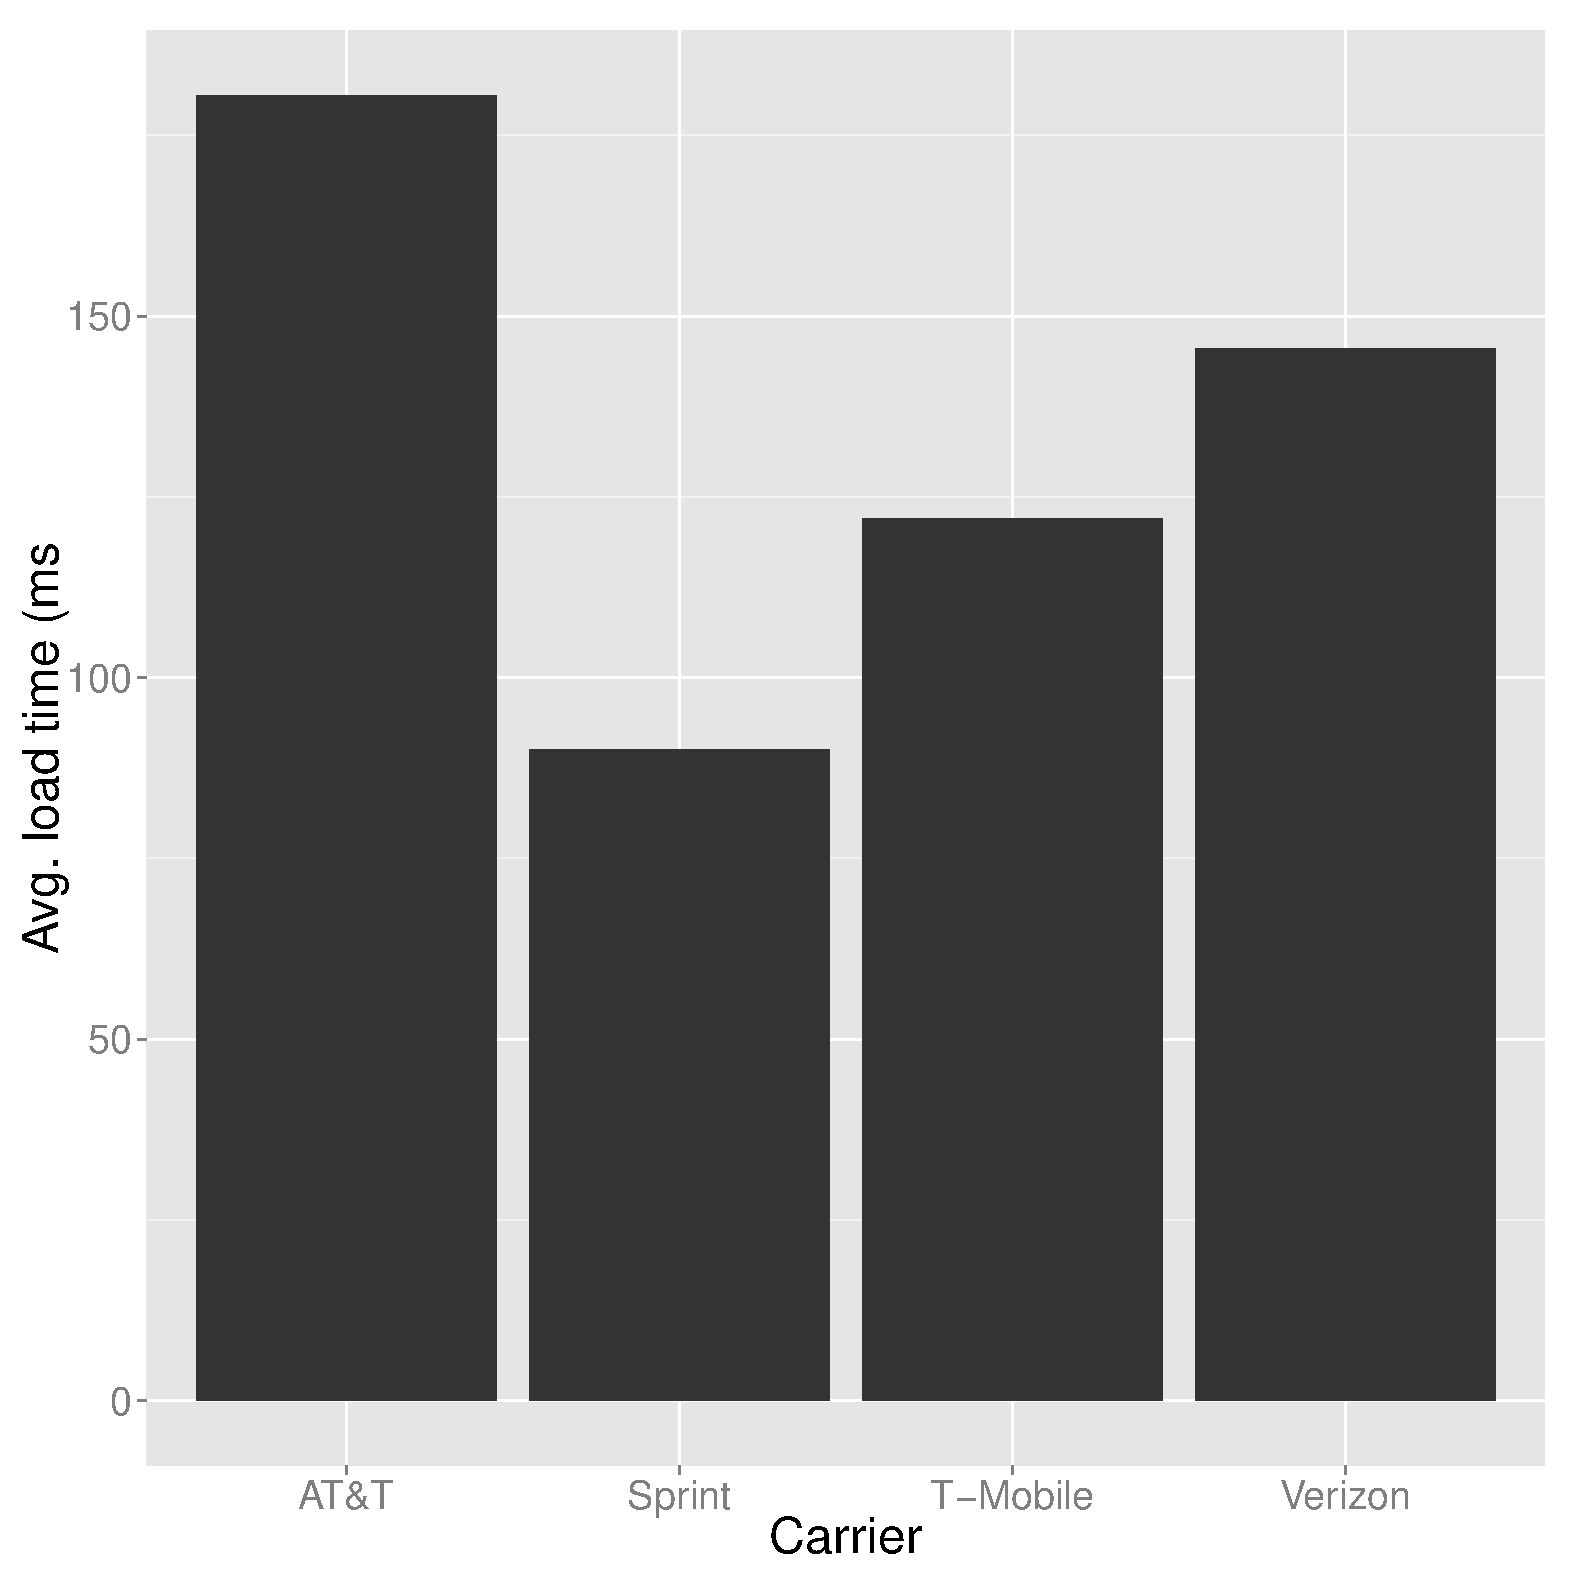
\includegraphics[width=4cm] {Images/dist1.pdf}}
		\caption{Visualization: Average \\ Load Times by Carrier
		 for BadApp}
		\label{fig:staplerX}
	\end{subfigure}
	
	\centering
	\begin{subfigure}{0.49\linewidth}
		{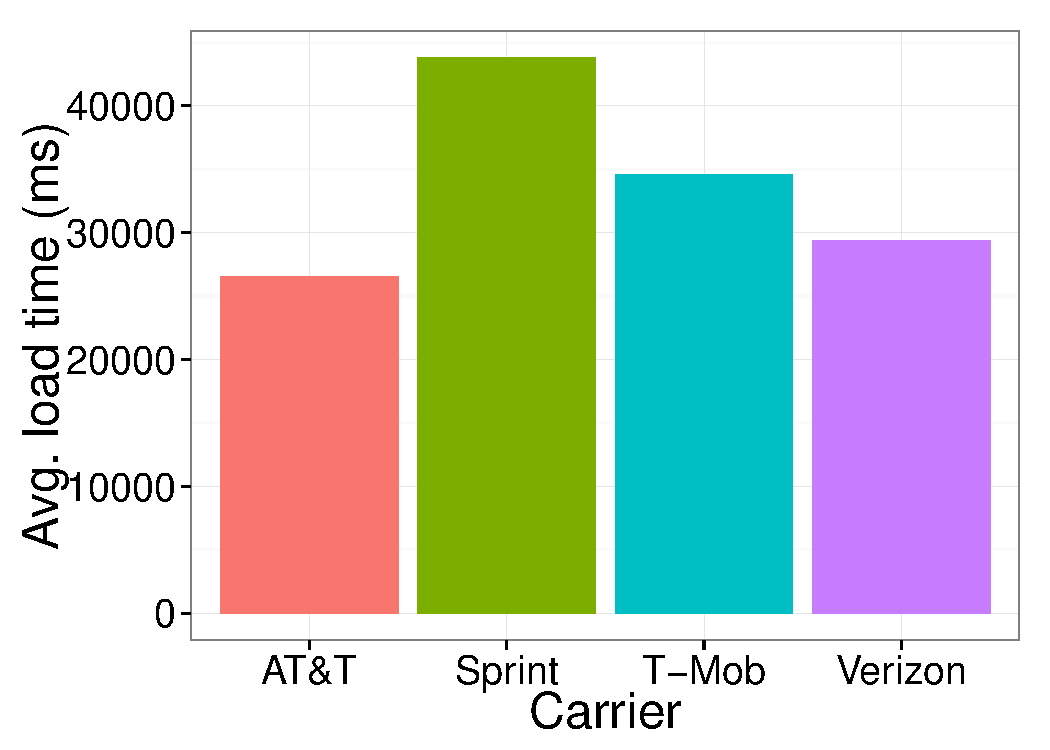
\includegraphics[width=4cm] {Images/dist2.pdf}}
		\caption{Scenario A: Average Load Times by Carrier}
		\label{fig:staplerX-a}
	\end{subfigure}
	\begin{subfigure}{0.49\linewidth}
		\centering
		{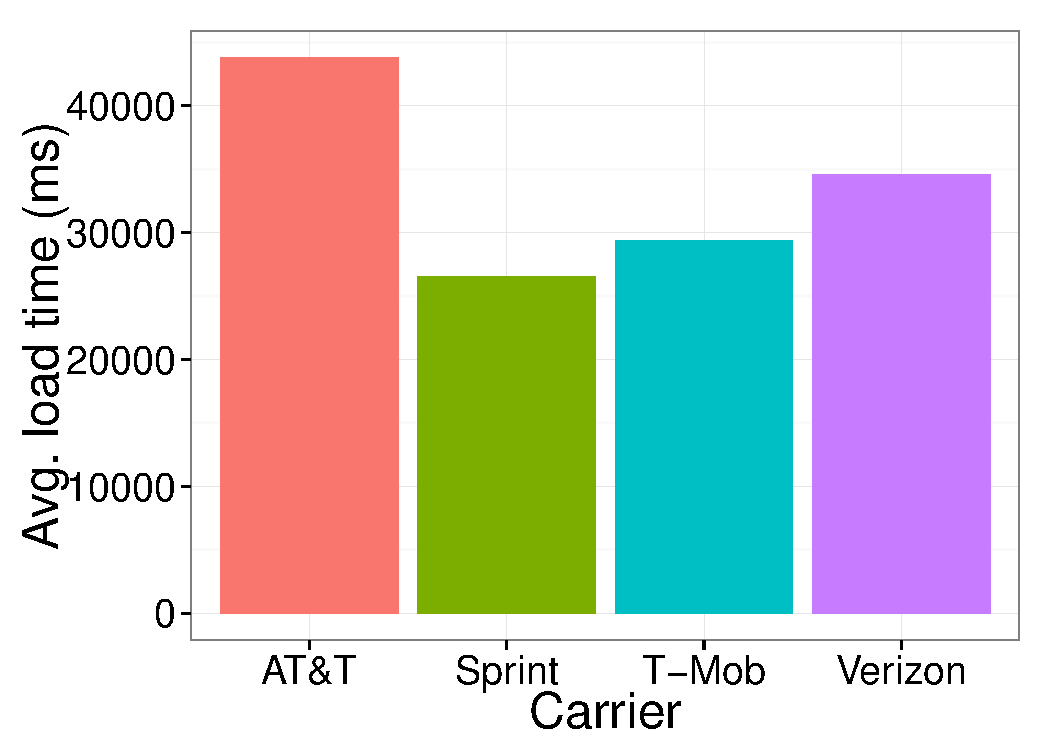
\includegraphics[width=4cm] {Images/dist3.pdf}}
		\caption{Scenario B: Average Load Times by Carrier}
		\label{fig:staplerX-b}
	\end{subfigure}
	\vspace{-10pt}
	\caption{Motivating Example}
	\label{fig:intro}
	\vspace{-10pt}
\end{figure}

As discussed previously, what might make one of these visualizations valuable depends on a host of factors.
In this work, we use a utility metric that is based on deviation.
Specifically, we posit that a visualization is {\em potentially ``interesting'' if it shows 
a trend in the subset of data selected by the analyst
(i.e., metrics about BadApp)
that deviates from the equivalent trend in the overall dataset (i.e., metrics
about all apps)}.
In our example, the visualization of load times by carrier, as shown in Figure
\ref{fig:staplerX}, would be valuable if the global trend for load times of all
apps showed the {\it opposite} trend (e.g. Figure \ref{fig:staplerX-a}).
However, the same visualization may be uninteresting if the load times of all apps
follow a similar trend (Figure \ref{fig:staplerX-b}).
% (a) utility of a visualization depends closely on the {\it query} posed by the user, i.e., subset of the data
% the user is interested in; as a result, trends in the queried data ({\it local trends}) are much more relevant 
% than global trends.
% (b) visualizations that show trends that are {\it unexpected or different are interesting}; specifically, we a 
% visualization is valuable {\em if it shows a local trend that deviates from the equivalent global trend}.
% Therefore, a visualization that shows the same trend in both, query $Q$ and the underlying data, is not valuable;
% on the other hand, a visualization that shows a different trend in query $Q$ compared to the underlying data 
% is highly valuable.
Due to the scale of data, most common visualizations show aggregate summaries of data
as opposed to individual records (e.g. average sales by state vs. sales of each store 
in every state).
Consequently, our current implementation of \SeeDB\ also limits recommended visualizations to those showing aggregate 
summaries of data.

Of course, there are a variety of other possible data-driven metrics for  quality or utility
of a visualization.
For instance, one might focus on visualizations that show order statistics or anomalies~\cite{kandel}. 
These would be important for spotting, for example unusual spikes in machine load.
Similarly, drawing upon the literature on data cubes, one might choose visualizations that highlight aggregates that
are unusual given the remaining values in the cube~\cite{sarawagi}.
Finally, one might choose to not aggregate any values but show correlations between attributes by plotting a random
sampling of datapoints.  Incorporating these other types of visualizations into our framework is an interesting
direction for future work.

Finally, we note that of the vision for \SeeDB\ has been described in a previous vision paper~\cite{DBLP:conf/vldb/Parameswaran2013}, but
that paper presented neither the specific visualization search techniques nor any evaluation.


% The majority of visualizations that are generated in visualization systems are based on aggregate summaries of the
% underlying data.
% As a result, the {\it trends} we study are the results of grouping and aggregation applied to a given dataset.


% Thus, the recommendation algorithm used by \SeeDB\ works as follows: given a dataset $D$ and a query $Q$
% indicating the subset of data of interest to the analyst, \SeeDB finds the visualizations of $Q$ that 
% show the highest deviation between trends in $Q$ and trends in $D$. 
% Specifically, \SeeDB considers visualizations that can be constructed via a combinations of grouping and 
% aggregation applied to $Q$.

\mpv{mention the 3 different settings in problem definition}.

\subsection*{Contributions}

In this paper, we demonstrate that we can build real systems that efficiently search for the most
interesting visualizations at interactive time scales.
Specifically, we describe two approaches to searching the space of possible visualizations.
In our first approach, we draw upon traditional multi-query optimization and OLAP literature to implement \SeeDB\ 
as a wrapper on top of a database system. Our goal was to study how far we can push existing systems to support a
\SeeDB-type workload.
\srm{revise the following, based on what we actually present in terms of UDFs vs a custom system}
In our second approach, we implement a system that  shares sequential scans and query results between visualizations, and 
employs statistical techniques to perform aggressive pruning based on intermediate results.
% SRM already said
%At its core, given a query $Q$ indicating the subset of data that the analyst is
%interested in, the goal of \SeeDB\ automatically {\em identifies and
%highlights to the analyst the most interesting views of the query results using
%methods based on deviation}.

The contributions of this paper are:
\begin{denselist}
%  \item We design \SeeDB as a system for data-driven visualization recommendations.
%  We explore and evaluate two distinct implementations of the system, one as a
%  wrapper around a database and another a custom solution (Section~\ref{sec:system_architecture}).
\item We describe a general deviation-based framework for evaluating the quality of a visualization,
and present and evaluate a specific metric that identifies aggregate dimensions in a dataset that
show maximal variation.  We develop two classes of optimizations to make such aggregates run fast 
in a conventional DBMS.
  \item The first set of techniques
  combine queries and aggregates to minimize the number of queries executed and 
  maximize the sharing of scans between queries, 
  including bin-packing~\cite{garey} algorithms and parallelization
  (Section~\ref{sec:dbms_optimizations}).
  \item The second set of techniques further optimize the process by adapting techniques 
  from both traditional confidence-interval-based~\cite{hoeffding1963probability} top-$k$ ranking and the
   multi-armed bandit problem~\cite{bandits} 
   to the problem finding the top-$k$ visualizations (Section~\ref{sec:in_memory_execution_engine}).
  \item We explore visualization pruning techniques based on data distribution
  to prune visualizations even before they are evaluated by the \SeeDB\ system 
  (Section~\ref{sec:pruning}).
  \item We evaluate the performance of our optimizations on a range of
  real and synthetic datasets and demonstrate the resulting 8--20X speedup 
  (Section~\ref{sec:experiments}). We also demonstrate that our algorithms
  improve performance without affecting utility of visualizations significantly.
  \item We present the results of a user study evaluating the recommendations produced by \SeeDB.
\end{denselist}




